\documentclass[11pt]{article}
\usepackage[margin=.8in]{geometry}
\usepackage{amsmath,amssymb,graphicx,hyperref}
\setlength{\parindent}{0pt}\setlength{\parskip}{6pt}
\begin{document}
\begin{center}{\Large Actual residual quotient dimension at most two}\\
23 November 2026 --- local unsigned Lean component evidence\end{center}
\textbf{Actual result.}
Let \(R=K[W]\) be the actual affine Weierstrass coordinate ring and \(I\) the
actual nonsingular target point ideal. Retain the accepted normalized function
and residual ideal construction under the original short-form, nonzero two
and ordinate, three paired nonsingular nodes and target-outside-support premises.
Lean derives
\[
 \dim_K(R/I^n)=n,\qquad
 \langle h\rangle=I^4J,\quad h\ne0,\qquad
 \dim_K(R/J)\le2.
\]
The actual quotients are finite dimensional. Neither the power dimension nor
the residual bound two is supplied as a premise
(PCC-20261123-6acf43) [pcc:unverified].
\begin{center}
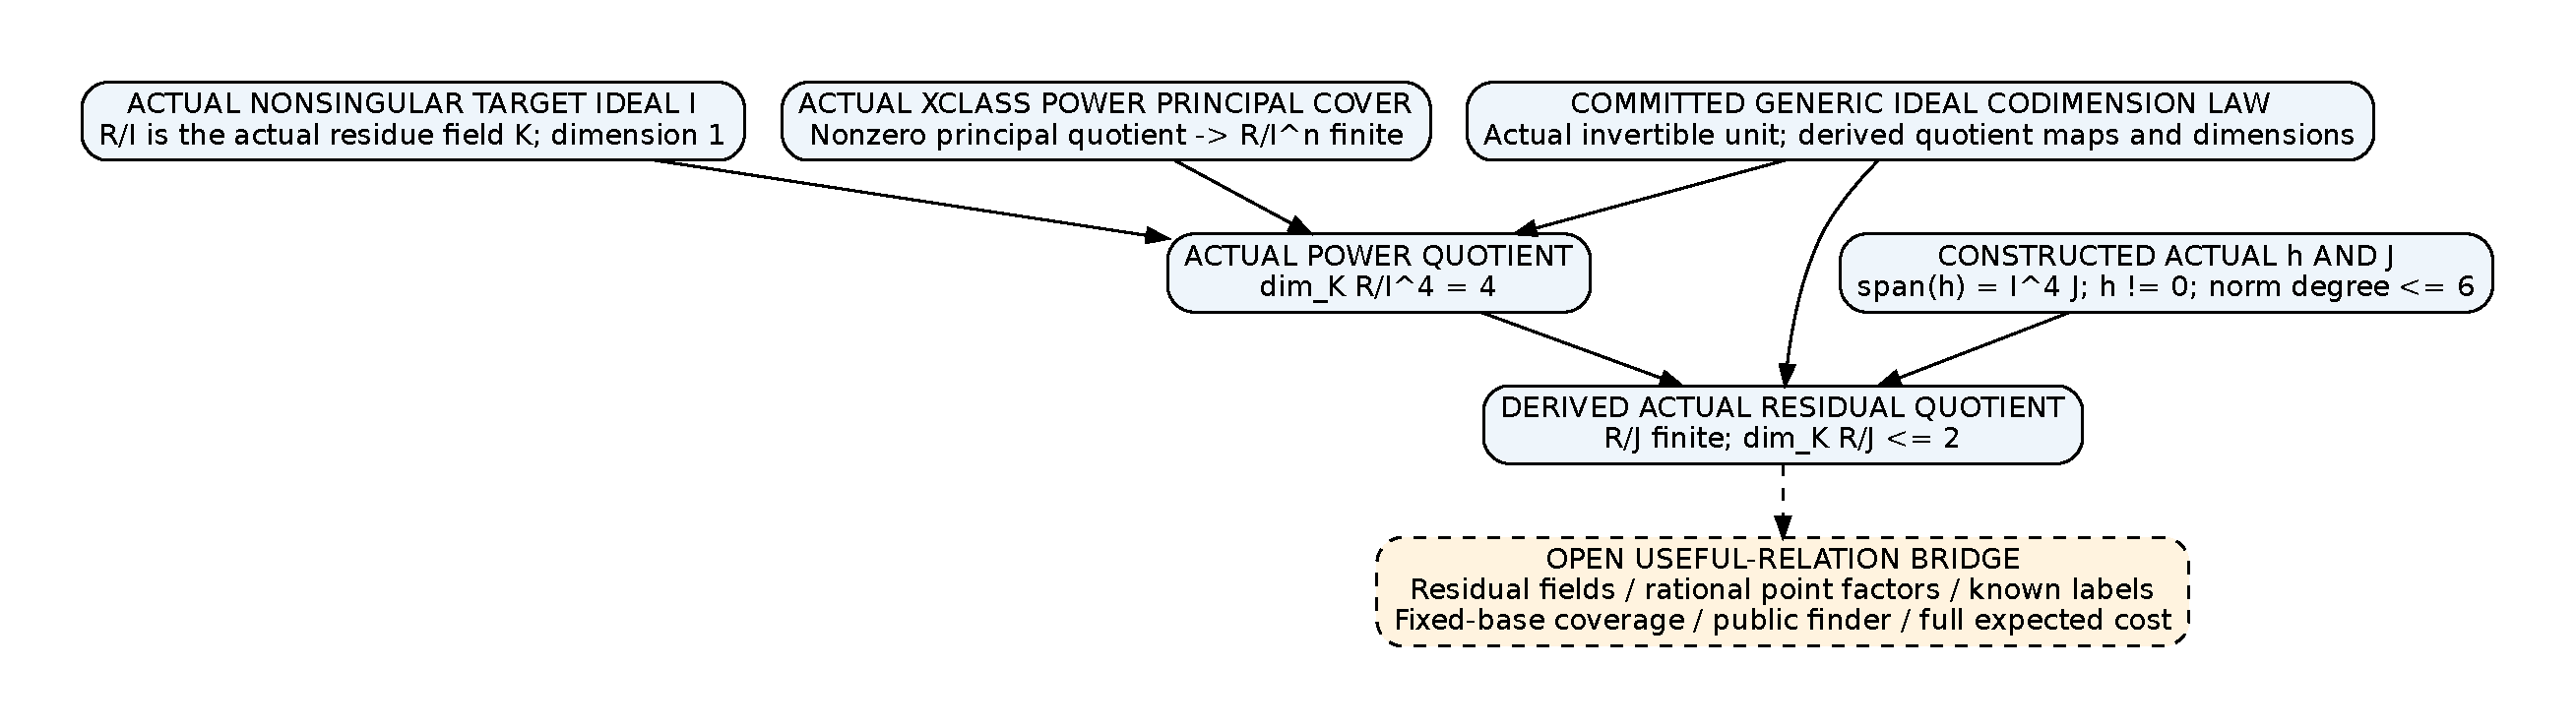
\includegraphics[height=5.15in,width=.96\linewidth,keepaspectratio]{residual-codimension-dependencies-001.pdf}
\end{center}
Solid arrows describe the checked algebraic implications. The dashed boundary
records a separate useful-relation obligation; dimension two alone does not
supply rational splitting or known scalar labels.
\newpage
\begin{center}{\Large Derived dimensions, exact checks and application boundary}\end{center}
\textbf{Actual point quotient and finiteness.}
The public actual point quotient algebra equivalence identifies \(R/I\) with
\(K\), giving dimension one. For every \(n\), the actual nonzero element
\((X-x_t)^n\) of the coordinate ring belongs to \(I^n\).
Its nonzero principal quotient is finite dimensional by the accepted norm
quotient theorem. The actual quotient surjection then makes \(R/I^n\) finite,
including \(n=0\) [pcc:unverified].

\textbf{Actual power and residual dimensions.}
The actual nonsingular point supplies an invertible fractional ideal unit
representing \(I\). The separately committed generic power theorem derives
\(\dim_K(R/I^n)=n\dim_K(R/I)=n\).
The actual fourth-power unit and product codimension theorem give
\[
 \dim_K(R/\langle h\rangle)=4+\dim_K(R/J).
\]
The principal quotient dimension equals the actual norm degree, at most six.
Thus \(\dim_K(R/J)\le2\). The proof explicitly transports finiteness across
\(\langle h\rangle=I^4J\) and derives the unit representing the actual ideal
power [pcc:unverified].

\textbf{Proof map and standing.}
Source073/build079/local038 checks191 statements, five new since186, exit zero,
zero warnings; all191 printed foundations are standard. The five declarations
use the namespace below:
\begin{center}\texttt{OrientationActualResidualCodimension}\end{center}
\begin{center}\begin{tabular}{l}
\texttt{point\_quotient\_finrank}\\
\texttt{point\_power\_quotient\_finite}\\
\texttt{point\_power\_quotient\_finrank}\\
\texttt{actual\_residual\_quotient\_bound\_two}\\
\texttt{actual\_residual\_witness\_two}
\end{tabular}\end{center}
PCC-20261123-6acf43 is unsigned local data, outside historical shared
Transport53/57 audit/fresh. Lean 4.35.0, exact Mathlib revision and 249 direct
input bindings are pinned. No unchanged full-project replay was run
[pcc:unverified].

\textbf{Generic owner and sources.}
Three committed owner components derive finite-algebra invertible-module
triviality, the actual module quotient equivalence and actual ideal product/power
codimensions. Their focused unchanged audits cover respectively two, two and
five theorems, zero failing, zero extra trusted. Public Mathlib Picard,
tensor-quotient, quotient-map and rank-nullity results are reused; no novelty
claim is made for this standard algebra. Primary-source paths and exact owner
commits are in the dependency receipts. KB access remained unavailable as
recorded in the journal [pcc:unverified].

\textbf{Preservation and next test.}
Rejected072/build078 exposes an ideal-power coercion error; accepted073 uses
an explicit ideal type. Unlaunched071 and administrative076/077 failures remain
exact. All old pinned reports, sources, raw logs and claims remain unchanged.
Next derive the actual group relation under an explicit residual point-factor
certificate, then evaluate fixed known-log base coverage. Residual field cases,
actual factor finding and complete expected bit cost remain separate.
\end{document}
